\section{Selected solvers}

In order to carry out the performance comparison, a set of solvers is required.
Implementing all the algorithms cited during the \ref{sec:classification}
section would be not only a huge task but also a non optimum one. The reason is
that some of the cited solvers already include a brief comparison against other
similar or popular solver.

After a deep review and study of Lambert's problem bibliography, the following
solvers were selected: \cite{gauss1809}, \cite{battin1984}, \cite{gooding1990},
\cite{avanzini2008}, \cite{arora2013}, \cite{vallado2013} and \cite{izzo2015}.
From now on, the first author of each solver together with its publication date
will be used to reference the algorithm.

In the sub-sections below these lines, a deep analysis on each one of these
solvers is made and the justification of its selection is presented to the
reader. The \textit{curves for the time of flight} are included too. These
provide the relation between the free-parameter and the non-dimensional time of
flight or the dependent variable.

\subsection{Gauss 1809}

The algorithm devised by Gauss in 1809 became very popular in its days. Gauss
developed an algorithm based on three observed angles to compute the orbit of
Ceres, see \cite{bevdatvs2021} and provided one for solving Lambert's problem.

His algorithm exploited the ratio between the sector triangle areas. By its
time, it was considered to be a great improvement within initial orbit
determination subject. However, the algorithm is also known for its low accuracy
when the transfer angle exceeds around 90 degrees although performs well for
lower transfer angles and times.

In this subsection, only the fundamental equations required for solving this
method will be presented. However, if reader wants to review the original work
made by Gauss, then refer to his famous book \citetitle{gauss1809}. A modern
revision of the problem was made by \cite{teets1999} using the original notation
when possible. Let us present in the following lines, the basic expressions for
the method devised by Gauss. However, here the background presented by
\cite{bate1971} is used.

The independent variable employed by Gauss is named $x$, while the dependent one
is $y$. These two variables are related via the so-called \textit{two equations
of Gauss}, being those:

\begin{equation}
x = \frac{w}{y^2} - s\quad\quad\quad
y = 1 + X(s + x)
\label{eq:gauss_equations}
\end{equation}

where in previous equation, the auxiliary variables are the semi-perimeter $s$
and a variable $w$ related with the non-dimensional transfer time:

\begin{equation}
s = \frac{\norm{\vec{r_1}} + \norm{\vec{r_2}}}{2 \sqrt{\norm{\vec{r_1}}\norm{\vec{r_2}} \cos{\left(\frac{\Delta \theta}{2} \right)}}} - \frac{1}{2}\quad\quad\quad
w = \frac{\mu \Delta t^2}{\left(2\sqrt{\norm{\vec{r_1}} \norm{\vec{r_2}}} \cos{\left(\frac{\Delta \theta}{2} \right)}\right)^3}
\end{equation}

Finally, $X$ is given by the expression developed in \cite{moulton1970}:

\begin{equation}
X = \frac{4}{3}\left(1 + \frac{6}{5}x + \frac{6 \cdot 8}{5 \cdot 7}x^2 + \frac{6 \cdot 8 \cdot 10}{5 \cdot 7 \cdot 9}x^3 + ...\right)
\end{equation}

\vspace{0.5cm}
\begin{figure}[h]
  \centering
  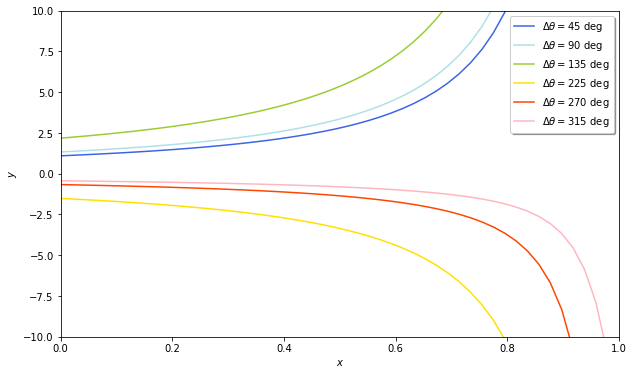
\includegraphics[width=\linewidth]{static/tof_curves/tof_gauss.png}
  \caption{Gauss 1809 time of flight curves for various transfer angles. This
  figure was obtained for $\rho=r_2/r_1=2$ with unitary $\mu$ and $\Delta t$.}
    \label{fig:tof_gauss}
\end{figure}

For solving the value of $x$, an initial guess about $y$ needs to be made, such
that $y_0=1.00$ for example. Then, the value of $x(y_0)$ is solved via equation
\ref{eq:gauss_equations} so a new value of $X(x)$ can be computed. Finally, a new
value of $y(x)$ is found. This value is compared with the initial one $y_0$ used
for the iteration. If $\norm{y - y_0} < \text{atol}$, then the method has
converged and the value for the free-parameter has been found. In figure
\ref{fig:tof_gauss}, the relation between the $x$ and $y$ parameter is shown
graphically for various transfer angles. The singular ones, such us any multiple
of $2\pi$ and $\pi$ have been omitted.

Finally, \cite{bate1971} suggests to use the semi-latus rectum for computing the
$f$ and $g$ functions, so the velocity vectors at the initial and final
positions can be obtained.

The decision to include this solver within the performance comparison was based
on two facts: the main one is its classic nature, so the solutions provided by
modern solvers can be better seen, the later is that \cite{sec:battin_solver}
improved this solver.


\subsection{Battin 1984}
\label{sec:batin_solver}

Batin is one of the author's who has devoted a lot of time reviewing and
studying the Lambert's problem. Chapters 6 and 7 from his book \citetitle{battin1999}
cover the whole geometry of the problem while provide a new algorithm following
the approach initiated by Gauss. Even if appearing in the book, this algorithm
is the result of a PhD thesis developed by Vaughan, under the supervision of
Battin, see \cite{vaughan1983}. The algorithm was published by both just a year
later in \cite{battin1984} and it is usually known as the Battin-Vaughan solver.

This new algorithm moves the singularity for transfer angles of $180$ degrees to
the less usual case of $360$ degrees. Although it no longer makes use of ratio
of sector to triangle areas, the notation used in the equations and the solution
procedures is quite similar to the solver devised by Gauss. No only that, this
solver is capable of fully working with all possible geometries and it is known
to have a better accuracy and robustness than Gauss one.

The so-called Battin's first and second equation, again following the ideas
introduced by Gauss, are given by expressions in \ref{eq:battin_equations}:

\begin{equation}
  x = \sqrt{\left(\frac{1 - l}{2} \right)^{2} + \frac{m}{y^2}} - \frac{1+l}{y^2}\quad\quad\quad
  y^3 - y^2 - h_1(x)y^2 - h_2(x) = 0
  \label{eq:battin_equations}
\end{equation}

where the auxiliary variables are given by \ref{eq:aux_battin}:

\begin{equation}
	\lambda = \pm \frac{\sqrt{s(s-c)})}{s}\quad\quad
	l = \left(\frac{1 - \lambda}{1 + \lambda}\right)^2\quad\quad\quad
	m = \frac{8\mu \Delta t^2}{s^3(1 + \lambda)^6}
	\label{eq:aux_battin}
\end{equation}

and the $h$ functions can be evaluated using expression \ref{eq:h_coeff}:

\begin{equation}
	h_1 = \frac{(l+x)^2(1 + 3x + \xi)}{(1+2x+l)(4x + \xi(3+x))}\quad
	h_2 = \frac{m(x-l+\xi)}{(1+2x+l)(4x + \xi(3+x))}
	\label{eq:h_coeff}
\end{equation}

being $\xi$ computed from a continued fraction defined in the original Battin's
article but simplified to:

\begin{equation}
  \xi(x) =
  \begin{cases}
	  \frac{4x(1 - \text{ATANR}(x))}{(3 +x)\text{ATANR}(x) - 3} &
	  \text{$x\neq0$}\\
	  5 & \text{$x = 0$}
  \end{cases}
\end{equation}

where the function $\text{ATANR}$ is an hypergeometric function defined as:

\begin{equation}
  \text{ATANR} = F(\frac{1}{2}, 1, \frac{3}{2}, -x) =
  \begin{cases}
	  \frac{\arctanh{\sqrt{-x}}}{\sqrt{-x}} & \text{$-1 < x < 0$}\\
	  1 & \text{$x = 0$} \\
	  \frac{\arctan{\sqrt{x}}}{\sqrt{x}} & \text{$x > 0$}
  \end{cases}
\end{equation}

following \cite{allen2015} article. This approach is cited here as
implementing continued fractions in a computer might be a bit tricky, leading to
non-optimized code. Modern computers do not struggle with the computations of
trigonometric functions as in the old days.

\vspace{0.5cm}
\begin{figure}[h]
  \centering
  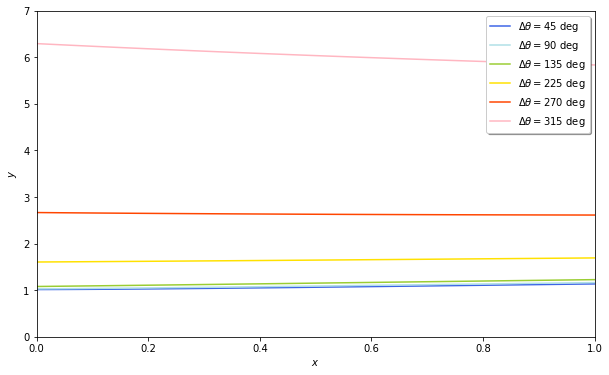
\includegraphics[width=\linewidth]{static/tof_curves/tof_battin.png}
  \caption{Battin 1984 time of flight curves for various transfer angles. This
  figure was obtained for $\rho=r_2/r_1=2$ with unitary $\mu$ and $\Delta t$.}
  \label{fig:tof_battin}
\end{figure}


Battin also improved previous equations at the end of his report to improve even
more the convergence of the method, so reader is encouraged to review them. The
implementation of the solver corresponds to these cited approach. The procedure
when solving the free-parameter $x$ is the same one as for the Gauss solver.
Curves for the time of flight are given figure \ref{fig:tof_battin}.

This solver was selected considering its enhancements over the Gauss one. Not
only that, it is one of the most moderns of the semi-latus rectum based solvers,
see subsection \ref{sec:p_solvers}.


\subsection{Gooding 1990}

The algorithm by \cite{gooding1990} was considered to have a high performance,
as claimed in performance reports of its days such us \cite{klumpp1999}. This is
the main reason behind its selection for the performance comparison.

Gooding's solver is based on the universal formulation branch, presented in
\ref{sec:universal_solvers}. This formulation enables to solve for elliptic,
parabolic or hyperbolic orbits without splitting the workflow into an excessive
amount of sections. Gooding's inherit from \cite{lancaster1970} solver and
dramatically improves its convergence and accuracy up to thirteen decimal
places.

The equation relating the canonical time of flight, named $T$ in Gooding's
article, and the free-parameter $x$ is complex. The equations collected by
\cite{torre2015} have been very useful and presented in \ref{eq:gooding_T}:

\begin{equation}
  \Delta t = 
  \begin{cases}
    4/3(1 - q^3) & \text{Parabolic solution}\\
    \sigma_x(f(x)) - q^3\sigma_x(q^2f(x)) & \text{Near-parabolic}\\
    \frac{2}{E(x)}\left(x - \lambda z(x) - \frac{d(x)}{y(x)}\right) & \text{Lancaster and Blanchard}
  \end{cases}
  \label{eq:gooding_T}
\end{equation}

Gooding's solver makes use of a bi-linear initial guess, which makes the initial
iteration value for the free-parameter to be closer to the final solution.
Together with the usage of a Halley's method, the convergence of the method is
quite fast. The construction of the velocity vectors is made using the radial
and tangential components. The curves for the time of flight, in figure
\ref{fig:tof_gooding}, are exactly the same ones as \cite{lancaster1970}, since
Gooding only devised and improved algorithm and did not introduce any additional
steps.

\vspace{0.5cm}
\begin{figure}[h]
  \centering
  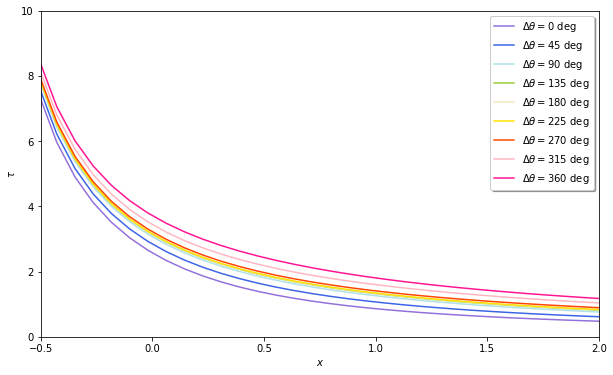
\includegraphics[width=\linewidth]{static/tof_curves/tof_gooding.png}
  \caption{Gooding 1990 time of flight curves for various transfer angles. This
  figure was obtained for $\rho=r_2/r_1=2$ with unitary $\mu$ and $\Delta t$.
  Only the direct transfer region is shown for the purposes of this work.}
  \label{fig:tof_gooding}
\end{figure}


\subsection{Avanzini 2008}

Among the different Lambert's problem solvers, the one devised by
\cite{avanzini2008} truly unleashes the geometry of the problem. This solver is
the very first of its branch within the set of eccentricity based ones, see
subsection \ref{sec:ecc_solvers}. By exploiting the conservation of the
eccentricity vector projection onto the chord one, it is able to solve for the
problem no matter the geometry of the orbit.

Avanzini's starts defining the fundamental eccentricity of the orbit $e_F$ (the
component along the chord direction) and the transverse one $e_T$. This is the
one which will be used as free-parameter. The relations given by
\ref{eq:ecc_avanzini} apply:

\begin{equation}
	e_F = \frac{\norm{\vec{r_1}} - \norm{\vec{r_2}}}{\norm{\vec{c}}}\quad\quad
	\norm{\vec{e}} = \sqrt{e_F^2 + e_T^2}
	\label{eq:ecc_avanzini}
\end{equation}

The free-parameter is defined as:

\begin{equation}
  x =
  \begin{cases}
    \frac{e_P e_H}{e_P + e_H}\log{\left(\frac{e_P(e_T + e_H)}{e_H(e_P - e_T)}\right)} & \text{if $\Delta \theta < \pi$}\\
    -e_P \log{\left(1 - \frac{e_T}{e_P} \right)} & \text{if $\Delta \theta > \pi$}
  \end{cases}
\end{equation}

where $e_P$, and $e_H$ can be computed using expressions \ref{eq:ecc_aux}:

\begin{equation}
  e_P = \sqrt{1 - e_F^2}\quad\quad\quad
  e_H = \sqrt{(e_\text{max}^2 - e_F^2)}\quad\quad
  e_\text{max} = \frac{-1}{\cos{\Delta \theta / 2}}
  \label{eq:ecc_aux}
\end{equation}

with all previous relations, it is possible to estimate the value of the
transverse eccentricity from the free-paramter $x$ by making use of equation
\ref{eq:ecc_T_avanzini}

\begin{equation}
  e_T =
  \begin{cases}
    e_P e_H \frac{X - 1}{e_p + e_H X} \text{if $\Delta \theta < \pi$}\\
    e_P \left(1 - \exp{\left(\frac{-x}{e_P} \right)} \right)
  \end{cases}
  \label{eq:ecc_T_avanzini}
\end{equation}

being $X$ defined as:

\begin{equation}
	X = \exp{\left(\left(\frac{1}{e_H} + \frac{1}{e_P} \right)x\right)}
\end{equation}

The starting value to be used for $x$ was imposed by Avanzini to be $x_0 = 0$.
The root solver declared by this author was the secant method, see subsection
\ref{sec:numerical_method}.

\vspace{0.5cm}
\begin{figure}[h]
  \centering
  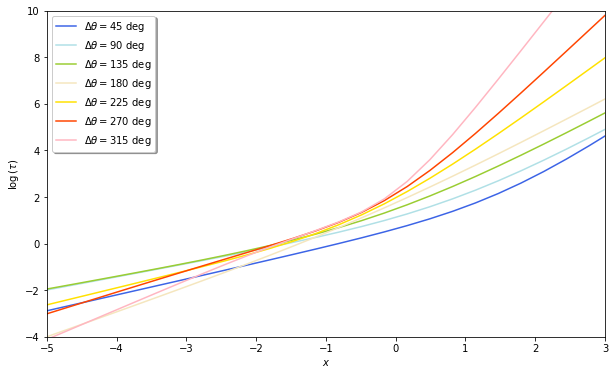
\includegraphics[width=\linewidth]{static/tof_curves/tof_avanzini.png}
  \caption{Avanzini 2008 time of flight curves for various transfer angles. This
  figure was obtained for $\rho=r_2/r_1=2$ with unitary $\mu$ and $\Delta t$.}
  \label{fig:tof_avanzini}
\end{figure}

Once the value of $x_0$ is known, the one for $e_T$ can be computed and then
the eccentricity of the orbit $e$, as the fundamental component is already
known. Therefore, to check if the value of $x_0$ is the right one, the current
time of flight and the one coming from the evaluation of Kepler's equation are
compared within some tolerance. As happens with other solvers, if the distance
between the two values is excessive, a correction is made to the free-parameter
and a new iteration begins till the method converges.

This solver was included due to its simplicity together with the fact of being
the first one of its class.

\subsection{Arora 2013}

Some years ago, \cite{arora2013} published a new Lambert's solvers based on a
cosine transformation. The new algorithm was strongly influenced by
\cite{bate1971} one and compared in performance against \cite{gooding1990} one
in Arora's publication. This solver belongs to the \ref{sec:universal_solvers}
set.

Arora introduced the $k$ free-paramter, which is related to the eccentric and
hyperbolic anomalies. The canonical time of flight can be computed as:

\begin{equation}
	\text{TOF} = S\sqrt{1 - k\tau}(\tau + (1 - k\tau)W)
\end{equation}

where the auxiliary parameters $\tau$, $S$ and $W$ are obtained via:

\begin{equation}
  S = \sqrt{\frac{(\norm{\vec{r_1}} + \norm{\vec{r_2}})^3}{\mu}}\quad\quad
  W = \frac{q}{\sqrt{m ^3}} - \frac{k}{m}\quad\quad
  m = 2 - k^2
\end{equation}

Avanzini improved the convergence of the method by converting some expressions
into series expansion- However, the core of this solver lies in the strong and
robust initial guess procedure devised by the author. Although based on a
rational-formulae (arbitrary initial guess), the solver rapidly converges in a
couple of iterations to the final solution.

The solution procedure is similar to Avanzini's solver, in the sense that
Kepler's equation is evaluated for various values of $k$ till it matches the
current time of flight.

The algorithm was also devised for working within the multi-revolution scenario
but as introduced early, the analysis of this region is out of the scope of this
work. Therefore, the curves for the time of flight for this solver presented in
figure \ref{fig:tof_arora} only show the direct transfer region.

\vspace{0.5cm}
\begin{figure}[h]
  \centering
  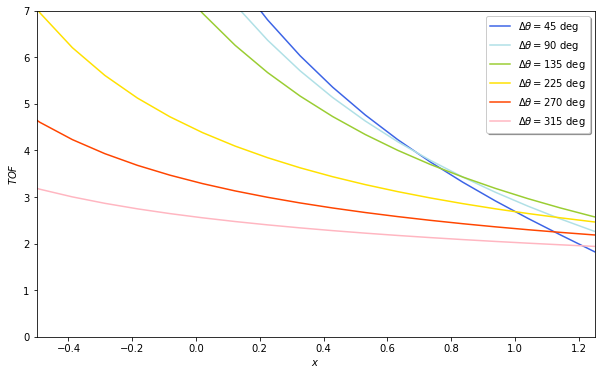
\includegraphics[width=\linewidth]{static/tof_curves/tof_arora.png}
  \caption{Arora 2013 time of flight curves for various transfer angles. This
  figure was obtained for $\rho=r_2/r_1=2$ with unitary $\mu$ and $\Delta t$.}
  \label{fig:tof_arora}
\end{figure}

The numerical method used by Arora is Halley's one and the subroutine for the
computation of the initial and final velocity vectors is made using the $f$ and
$g$ functions.


\subsection{Vallado 2013}

One of the most popular books about modern astrodynamics is the
\citetitle{vallado2013} by which also provides different pseudo-code for
implementing a variety of useful computer algorithms related with orbital
mechanics. One of these algorithms was an improved version of the
\cite{bate1971} universal one, for which Vallado imposed a bisection method. By
doing so, the method is ensured to converge no matter the type of orbit.

Vallado introduces the $\psi$ variable as the free-parameter. This variable is
related to the universal Kepler's equation via equation \ref{eq:tof_vallado}:

\begin{equation}
  t = \frac{\chi^3 c_3 + A \sqrt{y}}{\sqrt{\mu}}
  \label{eq:tof_vallado}
\end{equation}

where the variables $\chi$ and $y$ are given by:

\begin{equation}
  \chi = \sqrt{\frac{y}{c_2}}\quad\quad
  y = \norm{\vec{r_1}} + \norm{\vec{r_2}} + \frac{A(\psi + c_3 - 1)}{\sqrt{c_2}}
\end{equation}

and the transfer angle parameter $A$ is computed as:

\begin{equation}
  A = 
  \begin{cases}
    \sqrt{\norm{\vec{r_1}} \norm{\vec{r_2}} (1 + \cos{(\Delta \theta)})} & \text{if $\Delta \theta < \pi$}\\
    -\sqrt{\norm{\vec{r_1}} \norm{\vec{r_2}} (1 + \cos{(\Delta \theta)})} & \text{if $\Delta \theta > \pi$}\\
  \end{cases}
\end{equation}

In previous equations, the values for the $c_2$ and $c_3$ variables can be
computed using the corresponding Stumpff coefficients evaluated at a particular
value of $\psi$.

\vspace{0.5cm}
\begin{figure}[h]
  \centering
  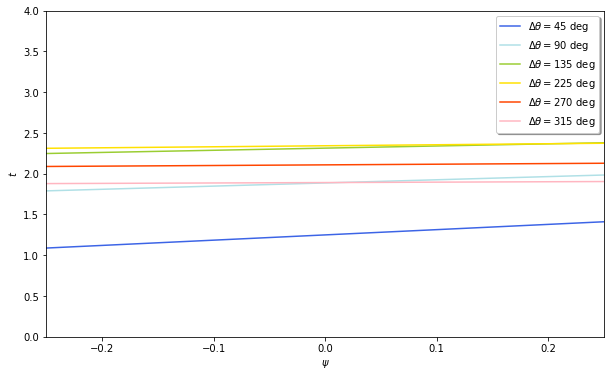
\includegraphics[width=\linewidth]{static/tof_curves/tof_vallado.png}
  \caption{Vallado 2013 time of flight curves for various transfer angles. This
  figure was obtained for $\rho=r_2/r_1=2$ with unitary $\mu$ and $\Delta t$.}
  \label{fig:tof_vallado}
\end{figure}

Similarly to other solvers, the goal is to iterate on the free-parameter till
the time computed using the universal Kepler's equation is equal to the expected
one imposed by the statement of the problem within some tolerance. Because this
method makes use of bisection, the solution is guaranteed to converge always.
However, a huge number of iterations is required for the solver to achieve
accurate results.

This method is belongs to the same branch as the one for \cite{arora2013}, see
the diagram from subsection \ref{sec:universal_solvers}. Therefore, Vallado's
solver was selected due to its simplicity against Arora's one so a performance
can be between them. 

\subsection{Izzo 2015}

The last of the solvers for this work is the one devised by \cite{izzo2015}.
This solver quickly became popular because it enhanced \cite{lancaster1970} and
\cite{gooding1990} ones by introducing one last change of variable. Not only
that, the Halley's method was upgraded to a Householder's one while the initial
guess made use of a linear approximation instead of a bi-linear one.

Izzo's solver belongs to the \ref{sec:universal_solvers} and names the
free-parameter $\xi$. This variable is related to Gooding's one $x$ via the
transformation given in \ref{eq:izzo_gooding}:

\begin{equation}
  \xi = 
  \begin{cases}
    \log{(1 + x)} & \text{if $M=0$}\\
    \log{\left(\frac{1+x}{1-x} \right)} & \text{if $M>0$}
  \end{cases}
  \label{eq:izzo_gooding}
\end{equation}

Regarding the non-dimensional time of flight, this variable is also modified
making use of expression \ref{eq:izzo_tof}:

\begin{equation}
  \tau = \log{(T)}
  \label{eq:izzo_tof}
\end{equation}

Izzo had to deal with the computation of the high-order derivatives of $\tau$
with respect to $\xi$. These are not provided here but can be checked in the
original report.

All previous modifications, ended up showing the relation between the
free-parameter and non-dimensional transfer angle which is presented in figure
\ref{fig:tof_izzo}.

\vspace{0.5cm}
\begin{figure}[h]
  \centering
  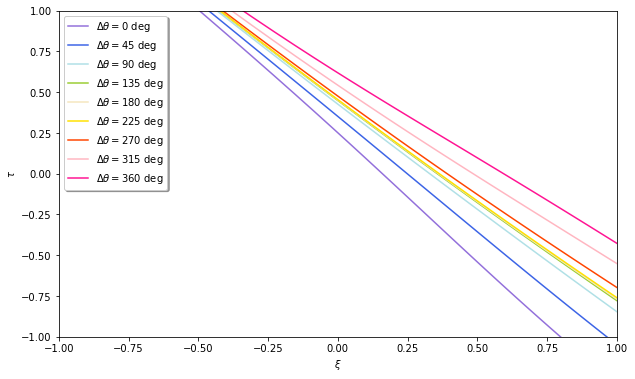
\includegraphics[width=\linewidth]{static/tof_curves/tof_izzo.png}
  \caption{Izzo 2015 time of flight curves for various transfer angles. This
  figure was obtained for $\rho=r_2/r_1=2$ with unitary $\mu$ and $\Delta t$.}
  \label{fig:tof_izzo}
\end{figure}
